\section{Abbreviations}

\begin{center}
\begin{tabular}{lll}
knowledge representation and processing & KRP & the general area of this course \\
knowledge representation language & KRL & a languages used in KRP \\
knowledge representation tool & KRT & a tool implementing a KPL and processing algorithms for it
\end{tabular}
\end{center}

\section{Motivation}

\subsection{Knowledge}

Human knowledge pervades all sciences including computer science, mathematics, natural sciences and engineering.
That is not surprising: ``science'' is derived from the Latin word ``scire'' meaning ``to know''.
Similarly, philosophy, from which all sciences derive, is named after the Greek words ``philo'' meaning loving and ``sophia'' meaning wisdom, and the for common ending ``-logy'' is derived from Greek ``logos'' meaning word (i.e., a representation of knowledge).

In regards to knowledge, computer science is special in two ways:
Firstly, many branches of computer science need to understand KRP as a prerequisite for teaching computers to do knowledge-based tasks.
In some sense, KRP is the foundation and ultimate goal of all artificial intelligence.%
\footnote{Indeed, a major problem with the currently very successful machine learning-based AI technology is that it remains unclear when and how it does KRP. That can be dangerous because it leads to AI systems recommending decisions without being able to explain why that decision should be trusted.}
Secondly, modern information technology enables all sciences to apply computer-based KRP in order to vastly expand on the domain-specific tasks that can be automated.
Currently all sciences are becoming more and more computerized, but most non-CS scientists (and many computer scientists for that matter) lack a systematic education and understanding of IT-KRP.
That often leads to bad solutions when domain experts cannot see which KRP solutions are applicable or how to apply them.

\subsection{Representation and Processing}

It is no coincidence that this course uses the phrase ``Representation and Processing''.
In fact, this is an instance of a universal duality.
Consider the following table of analogous concept pairs, which could be extended with many more examples:

\begin{center}
\begin{tabular}{l|l}
Representation & Processing \\
\hline
Static & Dynamic \\
Situation & Change \\
Be & Become \\
Data Structures & Algorithms \\
Set & Function \\
State & Transition \\
Space & Time
\end{tabular}
\end{center}

Again and again, we distinguish a static concept that describes/represents what is a situation/state is and a dynamic concept that describes how it changes.
If that change is a computer doing something with or acting on that representation, we speak of ``processing''.

It is particular illuminating to contrast KRP to the standard CS course on Data Structures and Algorithms (DA).%
\footnote{The course is typically called ``Algorithms and Data Structures'', but that is arguably awkward because algorithms can exist if there are data structure to work with. Compare my notes on that course in this repository, where I emphasize data structures much more than is commonly done in that course.}
Generally speaking, DA teaches the methods, and KRP teaches how to apply them.
Data structures are a critical prerequisite for representing knowledge.
But data structures alone do not capture what the data means (i.e., the knowledge) or if a particular representation makes any sense.
Similarly, algorithms are the critical prerequisite for processing knowledge.
But while algorithms can be systematically analyzed for efficiency, it is much harder to analyze if an algorithm processes knowledge correctly.
The latter requires understanding what the input and output data means.

Capturing knowledge in computers is much harder than developing data structures and algorithms.
It is ultimately the same challenge as figuring out if a computer system is working correctly --- a problem that is well-known to be undecidable in general and very difficult in each individual case.

%%%%%%%%%%%%%%%%%%%%%%%%%%%%%%%%%%%%%%%%%%%%%%%%%%%%%%%%%%%%%%%
\section{Components of Knowledge}

\subsection{Syntax and Semantics, Data and Knowledge}

Four concepts are of particular relevance to understanding knowledge.
They form a $2\times 2$-quadruple of concepts:

\begin{center}
\begin{tabular}{l|l}
Syntax & Data \\
\hline
Semantics & Knowledge
\end{tabular}
\end{center}

All four concepts are primitive, i.e., they cannot be defined in simpler terms.
All sciences have few carefully-chosen primitive on which everything builds.
This is done most systematically in mathematics (where primitives include set or function).
While mathematical primitives as well as some primitives in physics or CS are specified formally, the above four concepts can only be described informally, ultimately appealing to pre-existing human understanding.
Moreover, this description is not standardized --- different courses may use very different descriptions even they ultimately try to capture the same elusive ideas.

\textbf{Data} (in the narrow sense of computer science) is any object that can be stored in a computer, typically combined with the ability to input/output, transfer, and change the object.
This includes bits, strings, numbers, files, etc.

Data by itself is useless because we would have no idea what to do with it.
For example, the object $O=((49.5739143, 11.0264941), "2020-04-21T16:15:00CEST")$ is useless data without additional information about its syntax and semantics.
Similarly, a file is useless data unless we know which file format it uses.

\textbf{Syntax} is a system of rules that describes which data is \textbf{well-formed}.
For $O$ above the syntax could be ``a pair of (a pair of two IEEE double precision floating point numbers) and a string encoding of an time stamp''. 
For a file, the syntax is often indicated by the file name extension, e.g., the syntax of an \texttt{html} file is given in Section 12 of the current HTML standard\footnote{\url{https://html.spec.whatwg.org/multipage/}}.

Syntax alone is useless unless we know what the semantics, i.e., what the data means and thus how to correctly interpret and process the data.
For example, the syntax of $O$ allows to check that $O$ is well-formed, i.e., indeed contains two numbers and a timestamp string.
That allows rejecting ill-formed data such as $((49.5739143, 11.0264941), "foo")$.
The HTML syntax allows us to check that a file conforms to the standard.

\textbf{Semantics} is a system of rules that determines the meaning of well-formed data.
For example, ISO 8601 specifies that timestamp string refer to a particular date and time in a particular time zone.
Further semantics for $O$ might be implicit in the algorithms that produce and consume it: such as ``the first component of the pair contains two numbers between $0$ and $180$ resp. $0$ and $360$ indicating latitude resp. longitude of a location on earth''.
Semantics might be multi-staged, and further semantics about $O$ might be that $O$ indicates the location and time of the first lecture of this course.
Similarly, Section 14 of the HTML standard specifies the semantics of well-formed HTML files by describing how they are to be rendered in a web browser.

\textbf{Knowledge} is the combining of some data with its syntax and semantics.
That allows applying the semantics to obtain the meaning of the data (if syntactically well-formed and signaling an error otherwise).
In computer systems,
\begin{compactitem}
 \item data is represented using primitive data (ultimately the bits provided by the hardware) and encodings of more complex data (bytes, arrays, strings, etc.) in terms of simpler ones,
 \item syntax is theoretically specified using grammars and practically implemented in programming languages using data structures,
 \item semantics is represented using algorithms that process syntactically well-formed data,
 \item knowledge is elusive and often emerges from executing the semantics, e.g., rendering of an HTML file.
\end{compactitem}

\subsection{Semantics as Syntax Transformation}

In order to capture knowledge better in computer systems, we often use two syntax levels: one to represent the data itself and another to represent the knowledge.
These can be seen as input and output data.
In that case, semantics is a function that translates from the data syntax to the knowledge syntax, and knowledge is the pair of the data and the result of applying the semantics.
The following table gives some examples.

\begin{center}
\begin{tabular}{l|l|l}
Data syntax & Semantics function & Knowledge syntax \\
\hline
SPARQL query & evaluation & result set \\
SQL query & evaluation & result table \\
program & compiler & binary code \\
program expression & interpreter & result value \\ 
logical formula & interpretation in a model & mathematical object \\
HTML document & rendering & graphical representation 
\end{tabular}
\end{center}

Thus, the role of syntax vs. semantics may depend on the context: just like one function's output can be another function's input, one interpretation's knowledge can be another one's syntax.
For example, we can first compile a program into binary and then execute it to returns its value.

Such hierarchies of evaluation levels are very common in computer systems.
In fact, most state-of-the-art compilers are subdivided into multiple phases each further interpreting the output of the previous one.
Thus, if knowledge is represented in computers, it is invariably data itself but relative to a different syntax.

\subsection{Heterogeneity of Semantics and Knowledge}

While it is easy to design languages to represent data in general, it is very difficult to designing KRLs that capture the human-level quality of knowledge.
Over the last few decades, the KRP area in computer science has diversified into different subareas that approach this research problem in fundamentally different ways.
In fact, KRP in the very general sense of this course is usually not even studied by itself --- instead the subareas are so different, specialized, and large that they all sustain their respective university courses and research conferences.

This is related to the fact the data naturally comes in fundamentally different forms such as graphs, arrays, tables in the sense of relational databases, programs in a programming language, logical formulas, or natural language texts.
We speak of \textbf{heterogeneous} data.
These different forms of data are supported by highly specialized KPTs: graph databases, array databases, relational databases, package databases for programming languages, theorem databases for logics (e.g., the Isabelle Archive of Formal Proofs), databases of research papers (such as the arXiv), and so on.

All of these are very successful for their respective kind of data.
And all of them include specifications of semantics and KP algorithms that implement this semantics.
But it can very massively how the semantics is specified and implemented.
This has cause major practical problems for tool interoperability: many projects require data in multiple formats and algorithms from multiple tools.
But the respective tools are often islands that assume that all data is represented in the tool's language and users do not use outside tools.
Therefore, the import/export capabilities of the tools are often limited.

Moreover, transporting data across systems is usually ignorant of the semantics: while each tool takes relatively good care to implement the semantics correctly, there is much less certainty that the semantics is preserved when exchanging data across tools.
For a trivial example, consider a tool that measure length in inches vs. a tool that uses centimeters, both using floating point numbers for the data: if they exchange the data, i.e., just the numbers, they may mis-communicate the semantics.%
\footnote{Problems like this have been involved in major disasters such as the Mars Climate Orbiter.} 

This problem is not easy to fix though.
The heterogeneity of data and semantics is so extreme that it is, in some cases, an open theoretical problem how knowledge can be shared at all across tools.
The basic idea --- exchange the data in a way that preserves semantics --- can be difficult to implement if both tools use entirely different paradigms to specify semantics.

%%%%%%%%%%%%%%%%%%%%%%%%%%%%%%%%%%%%%%%%%%%%%%%%%%%%%%%%%%%%%%%
\section{The Tetrapod Model of Knowledge}

The Tetrapod model of knowledge is an ongoing research project by the instructors of this course.
A first publication was made in \cite{CFKR:tetrapod:19}.
The structure of this course will draw heavily on the Tetrapod model to get an overview of the different approaches to KPR and their interoperability problems.

\subsection{Five Aspects of Knowledge}

The Tetrapod model distinguishes five basic \textbf{aspects} of knowledge and KPR as described below.
For each aspect, there is a variety dedicated KRLs supported by highly optimized KPTs as indicated in the following table:

\begin{center}
\begin{tabular}{lll}
Aspect & KRLs (examples) & KPTs (examples) \\
\hline
ontologization & ontology languages (OWL), description logics (ALC) & reasoners, SPARQL engines (Virtuoso) \\
concretization & relational databases (SQL, JSON) & databases (MySQL, MongoDb) \\
computation & programming languages (C) & interpreters, compilers (gcc) \\
deduction & logics (HOL) & theorem provers (Isabelle) \\
narration & document languages (HTML, LaTeX) & editors, viewers
\end{tabular}
\end{center}

\textbf{Ontologization} focuses on developing and curating a coherent and comprehensive ontology of concepts.
This focuses on identifying the central concepts in a domain and their relations.
For example, a medical ontology would define concepts for every symptom, disease, and medication and then define relations for which symptoms and medications are related to which disease.

Ontologies typically abstract from the knowledge: they standardize identifiers for the concepts and spell out some properties and relations but do not try to capture all details of the knowledge.
Well-designed ontologies can capture exactly that different KPTs must share and can thus serve as interoperability layers between them.

While organization can use ontology languages such as OWL or RDF, the inherent complexity of formal objects in computer science and mathematics usually requires going beyond general purpose ontology languages (similar to how the programming languages underlying computer algebra systems usually go beyond general purpose programming languages).

\textbf{Concretization} uses languages based on numbers, strings, lists, and records to obtain concrete representations of datasets in order to store and query their properties efficiently.
Because concrete objects are so simple and widely used, it is possible and common to build concrete datasets on top of general purpose data representation languages and tools such as JSON or SQL.

\textbf{Computation} uses specification and programming languages to represent algorithmic knowledge.

\textbf{Deduction} uses logics and theorem provers  to obtain verifiable correctness.

\textbf{Narration} uses natural language to obtain texts are easy to understand for humans.
Because narrative languages are not well-standardized (apart from general purpose languages such as free text or \LaTeX), it is common to develop narrative libraries on top of ad-hoc languages that impose some formal structure on top of informal text, such as a fixed tree structure whose leafs are free text or a particular set of {\LaTeX} macros that must be used.
Narrative libraries can be classified based on whether entries are derived from publications (e.g., one abstract per paper in zbMATH) or mathematical concepts (e.g., one page per concept in $n$Lab).
%While these languages have multiple implementations, individual libraries usually involve specific encodings that are implemented only by a single tool.

%For example, an organization language might state only a function's type and properties.
%A computational treatment provides an efficient implementation, a deductive one proves the properties, a concretized one tables the function's values, and a narrative one documents the nature and purpose of the function.


\subsection{Relations between the Aspects}

The aspects can be visualized as the corners of tetrahedron with ontologization in the center and edges and faces representing solutions that mix two or three aspects as seen in Figure~\ref{fig:tetrapod}.

\begin{figure}[hbt]
\begin{center}
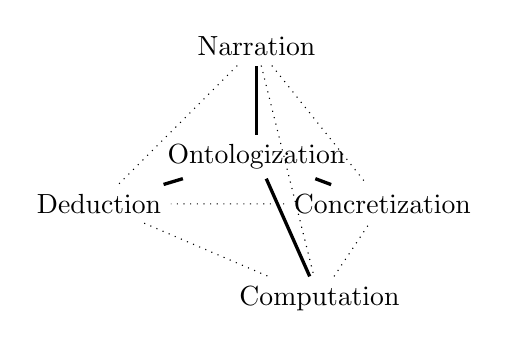
\begin{tikzpicture}[scale=4]
  \node (center) at (0,.15) {Ontologization};
  \node (left) at (.2,-.3) {Computation};
  \node (right) at (.4,0) {Concretization};
  \node (back) at (-.5,0) {Deduction};
  \node (up) at (0,.5) {Narration};

  \draw[very thick] (center) -- (left);
  \draw[very thick] (center) -- (right);
  \draw[very thick] (center) -- (back);
  \draw[very thick] (center) -- (up);
  \draw[dotted] (left) -- (right) -- (back) -- (left);
  \draw[dotted] (up) -- (left);
  \draw[dotted] (up) -- (right);
  \draw[dotted] (up) -- (back);
\end{tikzpicture}
\end{center}
\caption{Tetrapod model of knowledge}\label{fig:tetrapod}
\end{figure}

\begin{figure}[htb]\centering\footnotesize\setlength{\tabcolsep}{4pt}
\begin{tabular}{|l|llp{2.1cm}l|}\hline
       & \multicolumn{4}{c|}{characteristic} \\
Aspect &  objects & advantage & joint advantage of the other aspects & application \\\hline
deduction & formal proofs & correctness & ease of use & verification \\
computation & programs & efficiency & well-definedness & execution\\
concretization & concrete objects & tangibility & abstraction & storage/retrieval\\
narration & texts & flexibility & formal semantics & human understanding\\\hline
\end{tabular}
\quad
\begin{tabular}{|l|l|}\hline
Aspect pair & characteristic advantage \\\hline
ded./comp.  & rich meta-theory \\
narr./conc. & simple languages \\\hline
ded./narr.  & theorems and proofs \\
comp./conc. & normalization \\\hline
ded./conc.  & decidable well-definedness \\
comp./narr. & Turing completeness \\\hline
\end{tabular}
\caption{Shared properties and advantages of aspects}\label{fig:tetrapod2}
\end{figure}

Most approaches try to incorporate all or multiple aspects.
But all languages and tools tend to be heavily biased towards and optimized for a single one of the four corner aspects.
This is not due to ignorance but because each aspect provides characteristic advantages that are extremely hard to capture at once.
In fact, every combination of aspects shares characteristic advantages and disadvantages as sketched in Figure~\ref{fig:tetrapod2}.
For example, deductive and narrative definitions of a function involved well-definedness arguments, and a function defined by a concrete table is trivially well-defined, but a computational definition of a function may throw exceptions when running; but only the latter can store and compute functions efficiently.
Consequently, dedicated and mostly disjoint communities have evolved that have produced large aspect-specific datasets.

%\subsection{Aspect-Specific Datasets in Mathematics}
%
%A survey of the state of the art in aspects is huge.
%Figure~\ref{fig:libraries} gives an overview of important datasets just the domain of mathematics.
%We have also pre-published a draft of an extensive survey in \cite{CarFarSharBerKohMueRab:somss20}.
%
%Crucially, these disjoint projects overlap massively.
%For example, the concept of \emph{group} is defined in most proof assistants and computer algebra systems, concrete groups are part of multiple large libraries (e.g., as the main object of interest in the small groups libraries, or as symmetry groups arising from other objects), and has entries in most narrative libraries (e.g., with entries in Stacks and nLab).
%Despite the overwhelming practical need, at the moment there is little to no technology to integrate libraries across this overlap.
%The same effect is found in other domains.
%
%\begin{figure}[ht]\centering\small\def\cite#1{}
%  \begin{tabular}{| p{.3\textwidth} | p{0.55\textwidth}|}\hline
%  Dataset & Description and approximate size \\\hline\hline
%  \multicolumn{2}{|l|}{\textbf{Inference}} \\\hline
%  Theorem prover libraries  & ??? \\\hline
%  \multicolumn{2}{|l|}{\textbf{Computation} \hfill\strut\hfill {\tiny CAS = computer algebra system}} \\\hline
%  Mathematica & commercial CAS, $5k$ built-in functions, $150$k official examples\\\hline
%  Maple & commercial CAS, $5$k built-in functions \\\hline
%  GAP \cite{gap} & CAS for group theory, $10$k statements \\\hline
%  Singular \cite{singular:on} & CAS for polynomials, over $90$ libraries \\\hline
%  SageMath \cite{SageMath:on} & $1$k modules, bundled with $4$GB of CAS tools and libraries\\\hline
%  Modelica \cite{Modelica:on} & modeling language, $5$k built-in classes, $100$ open source libraries, $50$ commercial libraries up to $0.5$M equations \\\hline\hline % $10$ official, $>100$ open-source, $50$ commercial,
%  \multicolumn{2}{|l|}{\textbf{Concretization}} \\\hline
% OEIS \cite{OEIS:on} & $330$k integer sequences, $1$ TB; $0.3$M sequence identities in \cite{kwarc:datahost:on} \\\hline
%%  OEIS identities \cite{kwarc:datahost:on} & $0.3$M sequence identities, $2.5$ TB \\\hline
% various databases of graphs\cite{ConderCensuses:on, HartleyPolytopes:on, LeemansPolytopes:on, PotocnikCensuses:on, RoyleVT:on, WilsonET:on} & highly symmetric graphs, maps, polytopes, $30$ datasets, $2$M objects, $1$TB \\\hline
%  various databases of lattices \cite{KohLat:on, LeeLat:on, MalLat:on} & $7$ datasets, $17$G objects, $1.5$ TB \\\hline
%  findstat \cite{findstat} & combinatorial statistics and maps, $1.5$k objects \\\hline
%  SageMath databases \cite{SageDB:on} & $12$ datasets \\\hline
%  $L$-functions and modular forms \cite{lmfdb:on} & $80$ datasets, $1$G objects, $1$ TB \\\hline
%  Small Groups Library \cite{BeEiOBSmallGroups} & $450$M groups, $80$ MB \\\hline\hline
%  \multicolumn{2}{|l|}{\textbf{Narration}\hfill\strut\hfill {\tiny based on publications (P) or concepts (C)}} \\\hline
%  arXiv.org (P) & $300$k math preprints, most with {\LaTeX} sources\\\hline
%  zbMATH \cite{zbMATH:on} (P) & $4$M publication abstracts with semantic data, $30$M reference data, $1$M disambig. authors, $2.7$M full text links \\\hline % $1$M OA 
%  EuDML  \cite{EuDML:on} (P) & $260$k open full-text publications, digitized journal back issues \\\hline
%%  MathOverFlow & $\approx 1,1$M questions/answers, $\geq11$K answer authors \\\hline
%  Stacks project (C) & $6$k pages, semantically annotated, curated, searchable textbook \\\hline
%  $n$Lab (C) & $13$k pages on category theory and applications\\\hline
%  SMGloM glossary (C) & $1$k modules, $2$k concepts, $4.5$k multi-lingual verbalizations in English \\\hline\hline %  (100\%), German (90\%), Chinese (10\%)
%  \multicolumn{2}{|l|}{\textbf{Organization}} \\\hline
%  swMATH \cite{swMATH:on} & $25$k software records with $300$k links to $180$k publications \\\hline
%  Wikidata  \cite{wikidata:on} & $34$GB linked data, $4$k formulas, interlinked with named theorems, persons, publications \\\hline
%  DLMF & $500$ special mathematical functions, $10$k formulas \\\hline
%  OpenMath CDs \cite{openmath} & curated reference points for $1.5$k concepts \\\hline
%  LATIN atlas \cite{CHKMR:latinabs:11,LATIN:online} & modular definitions of logics, $1$k modules \\\hline
%  Formal Abstracts  \cite{fabstracts} & formal definitions for all concepts used by multiple authors of mathematical papers (planned) \\\hline
%  \oaf interface library & as obtained in \oaf WP 2.6\\\hline
%\end{tabular}
%  \caption{Representative examples of large libraries by aspect}\label{fig:libraries}
%\end{figure}
